\section{Root Cause Analysis in Cloud-Native Architectures}
\label{sec:root_cause_analysis}

According to classical reliability engineering literature---notably defined by researchers such as Robert J. Latino et al. and Duke Okes, building upon the U.S. Department of Energy guidelines---Root Cause Analysis (RCA) is a structured, evidence-based process designed to identify the underlying physical and systemic causes of a problem, moving beyond the superficial mitigation of symptoms \cite{latino_2011, okes_2019}. This diagnostic framework serves as a critical organizational learning mechanism aimed at understanding exactly why an adverse event occurred, distinguishing mere symptoms from the actual root causes to effectively prevent future recurrences \cite{groot_2021}. Unlike basic \textit{troubleshooting}---which often consists of reactive, ad-hoc patching aimed at rapidly restoring the system state---modern RCA demands a rigorous diagnostic phase characterized by continuous data collection and deterministic verification \cite{latino_2011}. Furthermore, contemporary literature emphasizes a ``systems thinking'' approach, warning that relying on simplified linear narratives or failing to alter the complex environment where the anomaly initially emerged will inevitably allow the adverse events to repeat \cite{groot_2021}.

\subsection{Observability as the Foundation for RCA}

In cloud-native environments, the ephemeral nature of containers orchestrated by Kubernetes obliterates local evidence when pods fail or are evicted \cite{barata_2026}. Consequently, executing a statistically sound RCA requires the telemetry pipeline to act as an uninterrupted, automated evidence preservation mechanism \cite{barata_2026}. 

\begin{figure}[htbp]
  \centering
  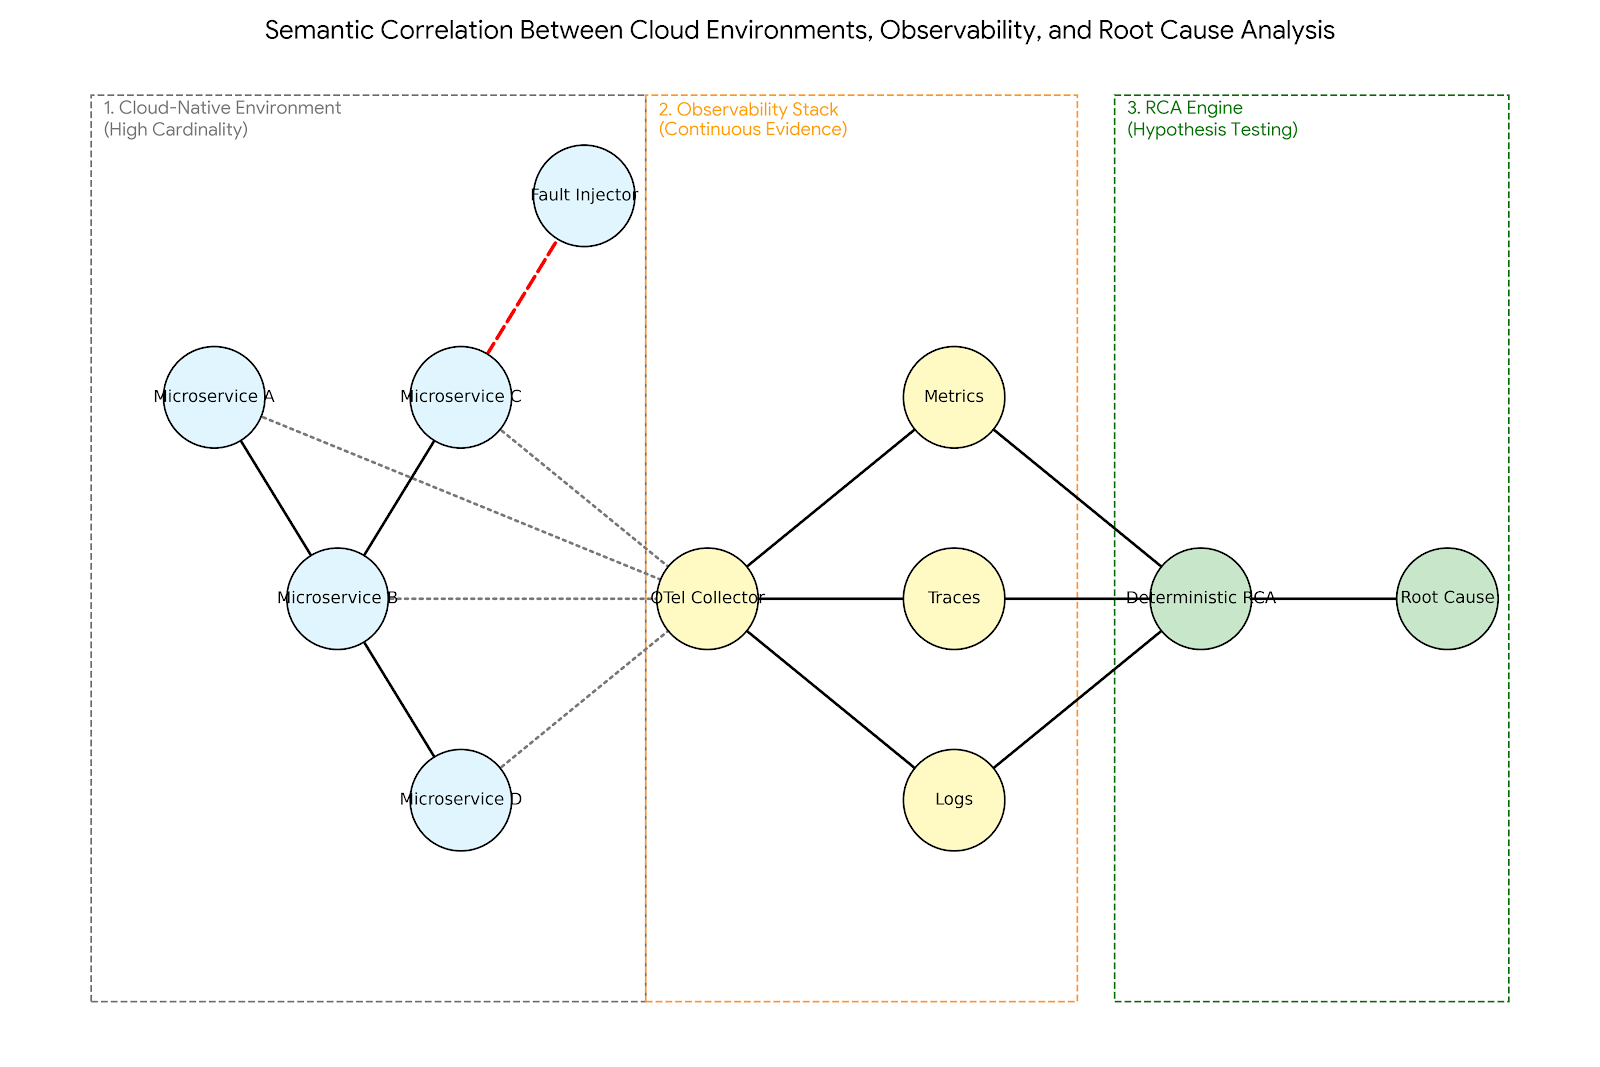
\includegraphics[width=1.0\textwidth]{images/observability/rca_observability_panorama.png}
  \caption{Semantic correlation between the Cloud-Native Environment, the Observability Stack, and the Deterministic RCA Engine.}
  \label{fig:rca_observability_panorama}
\end{figure}

As depicted in Figure~\ref{fig:rca_observability_panorama}, bridging the gap between a high-cardinality cloud environment and deterministic diagnosis requires a unified observability stack that correlates metrics, distributed traces, and logs. This architecture allows an algorithmic RCA agent to replace human intuition by traversing the telemetry graph and mathematically isolating the origin of the anomaly, thus mitigating the cognitive fatigue and time pressure typically placed on Site Reliability Engineers (SREs).

\subsection{Evaluation of Modern RCA Approaches}

The increasing complexity of microservice ecosystems has driven the evolution of RCA methodologies beyond traditional rule-based and manual techniques \cite{barata_2026}. Modern approaches leverage advanced computational paradigms, each with distinct strengths and weaknesses:

\begin{itemize}
    \item \textbf{Graph-Based Techniques:} These methods model the system topology and communication pathways as graphs to trace fault propagation \cite{brandon_2020}. \textit{Strengths:} They provide highly interpretable visualizations of cascading failures and effectively capture structural dependencies \cite{brandon_2020, barata_2026}. \textit{Weaknesses:} They often struggle with the dynamic, constantly shifting topologies of Kubernetes clusters and can be computationally expensive to maintain and query in real-time \cite{barata_2026}.
    
    \item \textbf{Causal Inference and Statistical Methods:} Algorithms such as the PC algorithm or Granger causality tests evaluate time-series data to mathematically distinguish causation from mere correlation \cite{ikram_2022, wang_2024}. \textit{Strengths:} They offer a rigorous mathematical foundation capable of identifying hidden root causes without relying on predefined rules, filtering out ``noisy neighbors'' effectively \cite{ikram_2022}. \textit{Weaknesses:} Traditional causal discovery algorithms often require an exponential number of conditional independence tests, making them impractically slow for large-scale microservice architectures unless optimized \cite{ikram_2022}.
    
    \item \textbf{Reinforcement Learning (RL):} RL models interact with the system environment to learn optimal troubleshooting policies through trial and error (rewards) \cite{barata_2026}. \textit{Strengths:} They exhibit high adaptability to the complex, variable structures of microservices and require very little prior domain knowledge \cite{barata_2026, wang_2024}. \textit{Weaknesses:} Defining an accurate reward function is complex, and the initial training phase can be resource-intensive \cite{barata_2026}.
    
    \item \textbf{Large Language Models (LLMs) and Agents:} Recent frameworks utilize LLMs to parse unstructured logs, trace spans, and generate diagnostic reasoning \cite{yao_2024, tang_2025, zhang_2026}. \textit{Strengths:} They excel at cross-modal semantic understanding, dramatically reducing the need for manual feature engineering \cite{zhang_2026}. \textit{Weaknesses:} LLMs suffer from limited exploration diversity, vulnerability to hallucinations, and heavy reliance on large-scale models that result in slow inference times, making them difficult to apply for sub-second, real-time remediation \cite{yao_2024, zhang_2026}.
\end{itemize}

Given the high dynamicity, scale, and multi-modal nature of Kubernetes environments, a hybrid approach that integrates Causal Inference with Reinforcement Learning has proven to be the most adequate \cite{barata_2026, wang_2024}. It overcomes the static limitations of pure graph methods and the slow inference of LLMs while maintaining mathematical determinism.

\subsection{The MRCA Framework: Metric-Level Root Cause Analysis}

To address the limitations of coarse-grained (service-level) localization and single-modality bottlenecks, Wang et al. (2024) proposed the \textit{Metric-level Root Cause Analysis for Microservices via Multi-Modal Data} (MRCA) framework \cite{wang_2024}. This architecture is utilized as the methodological core for the experimental evaluation in this thesis.

The MRCA framework operates through three highly optimized phases \cite{wang_2024}:

\begin{enumerate}
    \item \textbf{Multi-modal Data Feature Extraction:} MRCA integrates traces, logs, and metrics to capture a comprehensive view of the system \cite{wang_2024}. It utilizes the Drain parser to extract static templates from unstructured logs and calculates their frequencies, while concurrently extracting latency distributions from distributed traces \cite{wang_2024}.
    
    \item \textbf{Anomaly Detection via VAE:} Instead of feeding all data directly into the RCA engine—which causes computational bloat—MRCA employs a Variational Autoencoder (VAE) trained on normal multi-modal time-series data \cite{wang_2024}. During runtime, the VAE computes reconstruction probabilities; significant deviations trigger alerts \cite{wang_2024}. This filters out normal services and ranks the abnormal ones, passing only highly suspicious candidates to the next phase \cite{wang_2024}.
    
    \item \textbf{Root Cause Localization via Causal Inference and Q-Learning:} For the suspected services, MRCA applies the Granger causality algorithm to construct a causal graph based on metric data \cite{wang_2024}. Because evaluating all possible metric combinations is excessively time-consuming, MRCA introduces a Q-learning (Reinforcement Learning) agent to formulate a dynamic termination strategy \cite{wang_2024}. The agent assesses the complexity of the graph and the accuracy of the RCA to optimally halt the expansion of the causal graph \cite{wang_2024}. Finally, a pruning strategy removes descendant nodes, isolating the root cause at the specific metric level (e.g., isolating a memory leak indicator rather than just flagging the entire service) \cite{wang_2024}.
\end{enumerate}

By dynamically terminating the causal analysis and pinpointing faults at the metric level, MRCA provides SREs with precise, actionable intelligence, vastly outperforming traditional service-level diagnostics in both accuracy and computational efficiency \cite{wang_2024}.